\section{Component View}
Nella figura \ref{fig:ComponentDiagram_iterazione2} è riportato il diagramma a componenti relativo alle modifiche introdotte nell'iterazione 2. In particolare, è possibile notare le interfacce introdotte e la struttura dei componenti lato server e client.

\begin{figure}[h!]
	\centering
	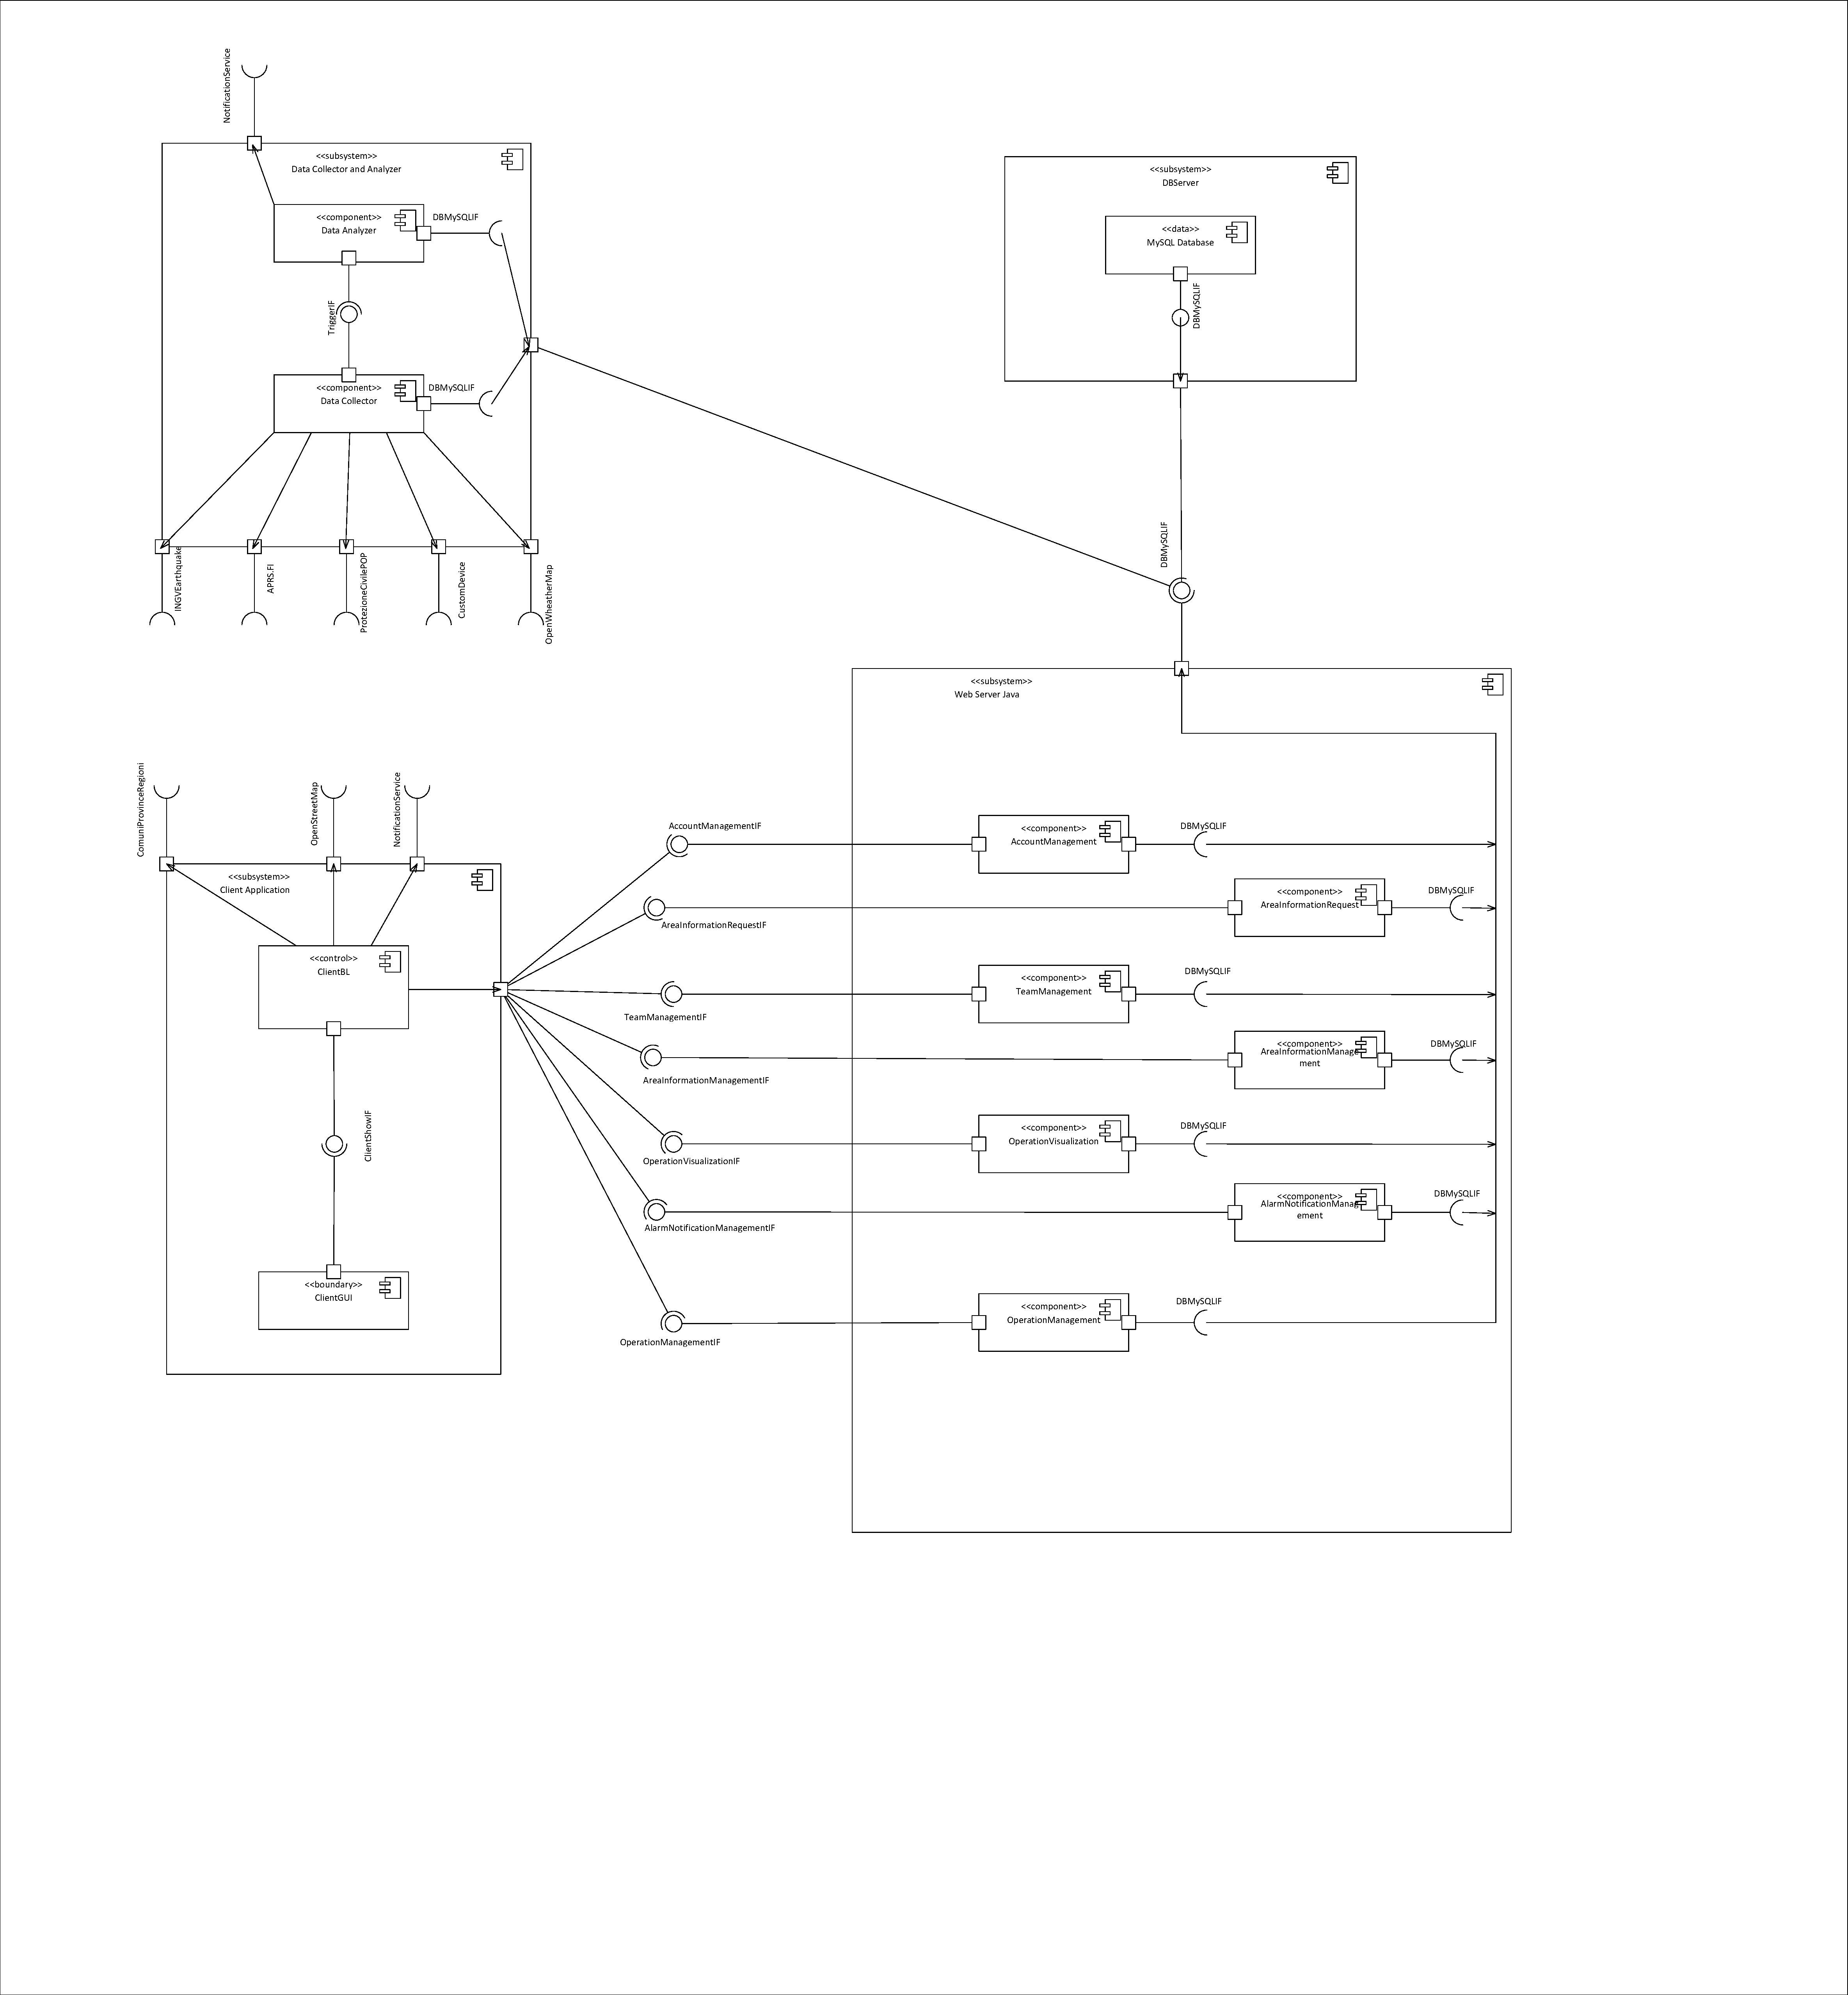
\includegraphics[width=1\linewidth]{./Iterazione 2/OtherFiles/UML - Component View}
	\caption{Component Diagram.}
	\label{fig:ComponentDiagram_iterazione2}
\end{figure}

\clearpage

Di seguito sono riportate le specifiche delle strutture dati \textit{UserDTO} e \textit{TeamDTO} (\Fig\ref{fig:ClassDiagramDTO_iterazione2}). Essi sono utilizzati per definire il formato dei dati scambiati tra l'applicazione client e il server. In particolare, si noti che il campo password nello \textit{UserDTO} è solamente valorizzato dall'app client nell'inserimento di un nuovo utente. Tuttavia, non viene mai inviato dal server al client.  

\begin{figure}[h!]
	\centering
	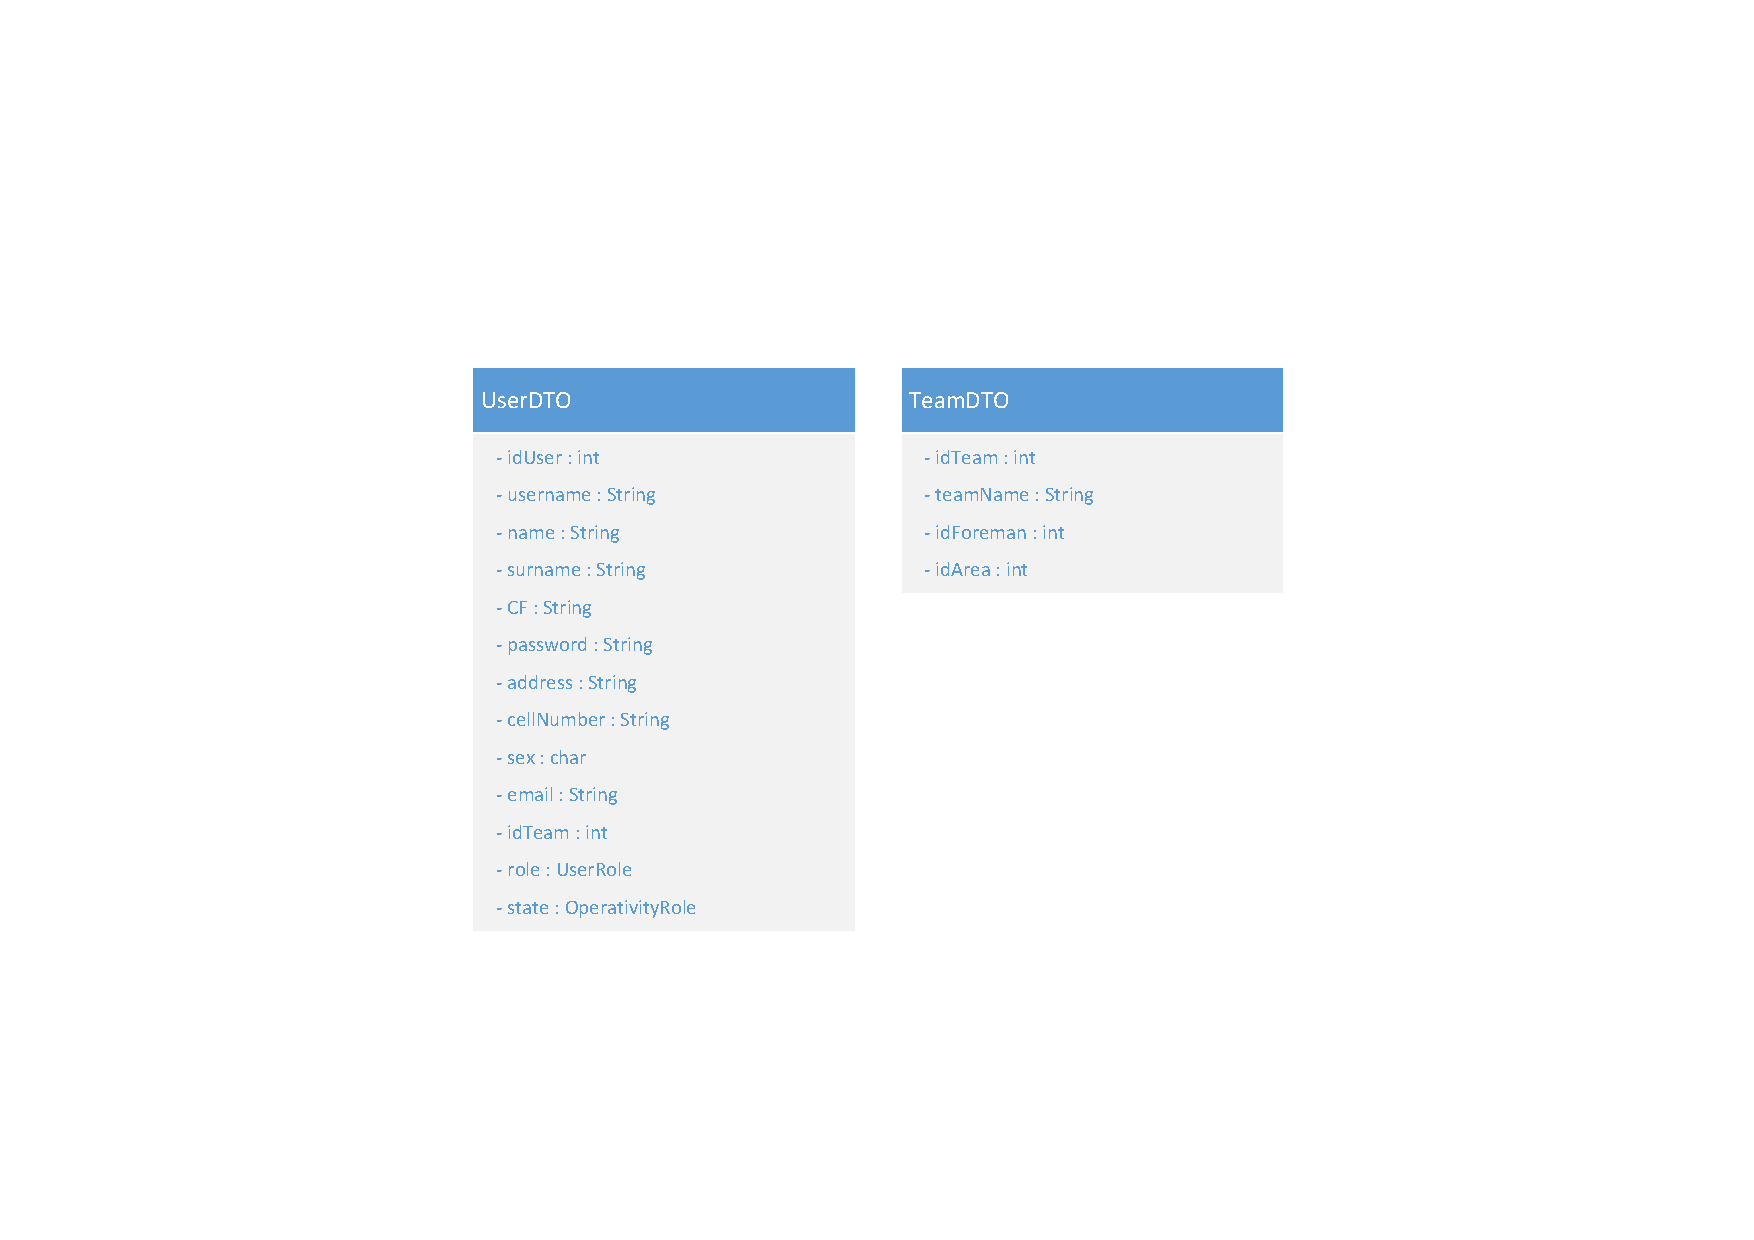
\includegraphics[width=1\linewidth]{./Iterazione 3/OtherFiles/DTOSpecification}
	\caption{Class Diagram UserDTO e TeamDTO}
	\label{fig:ClassDiagramDTO_iterazione2}
\end{figure}

\clearpage

\section{Interface and Packages Diagram}
Nella \Fig\ref{fig:InterfaceDiagram_iterazione2} è rappresentato il diagramma delle interfacce e dei package, nel quale è stata specificata anche la firma delle interfacce introdotte nell'iterazione 2.

\begin{figure}[h]
	\centering
	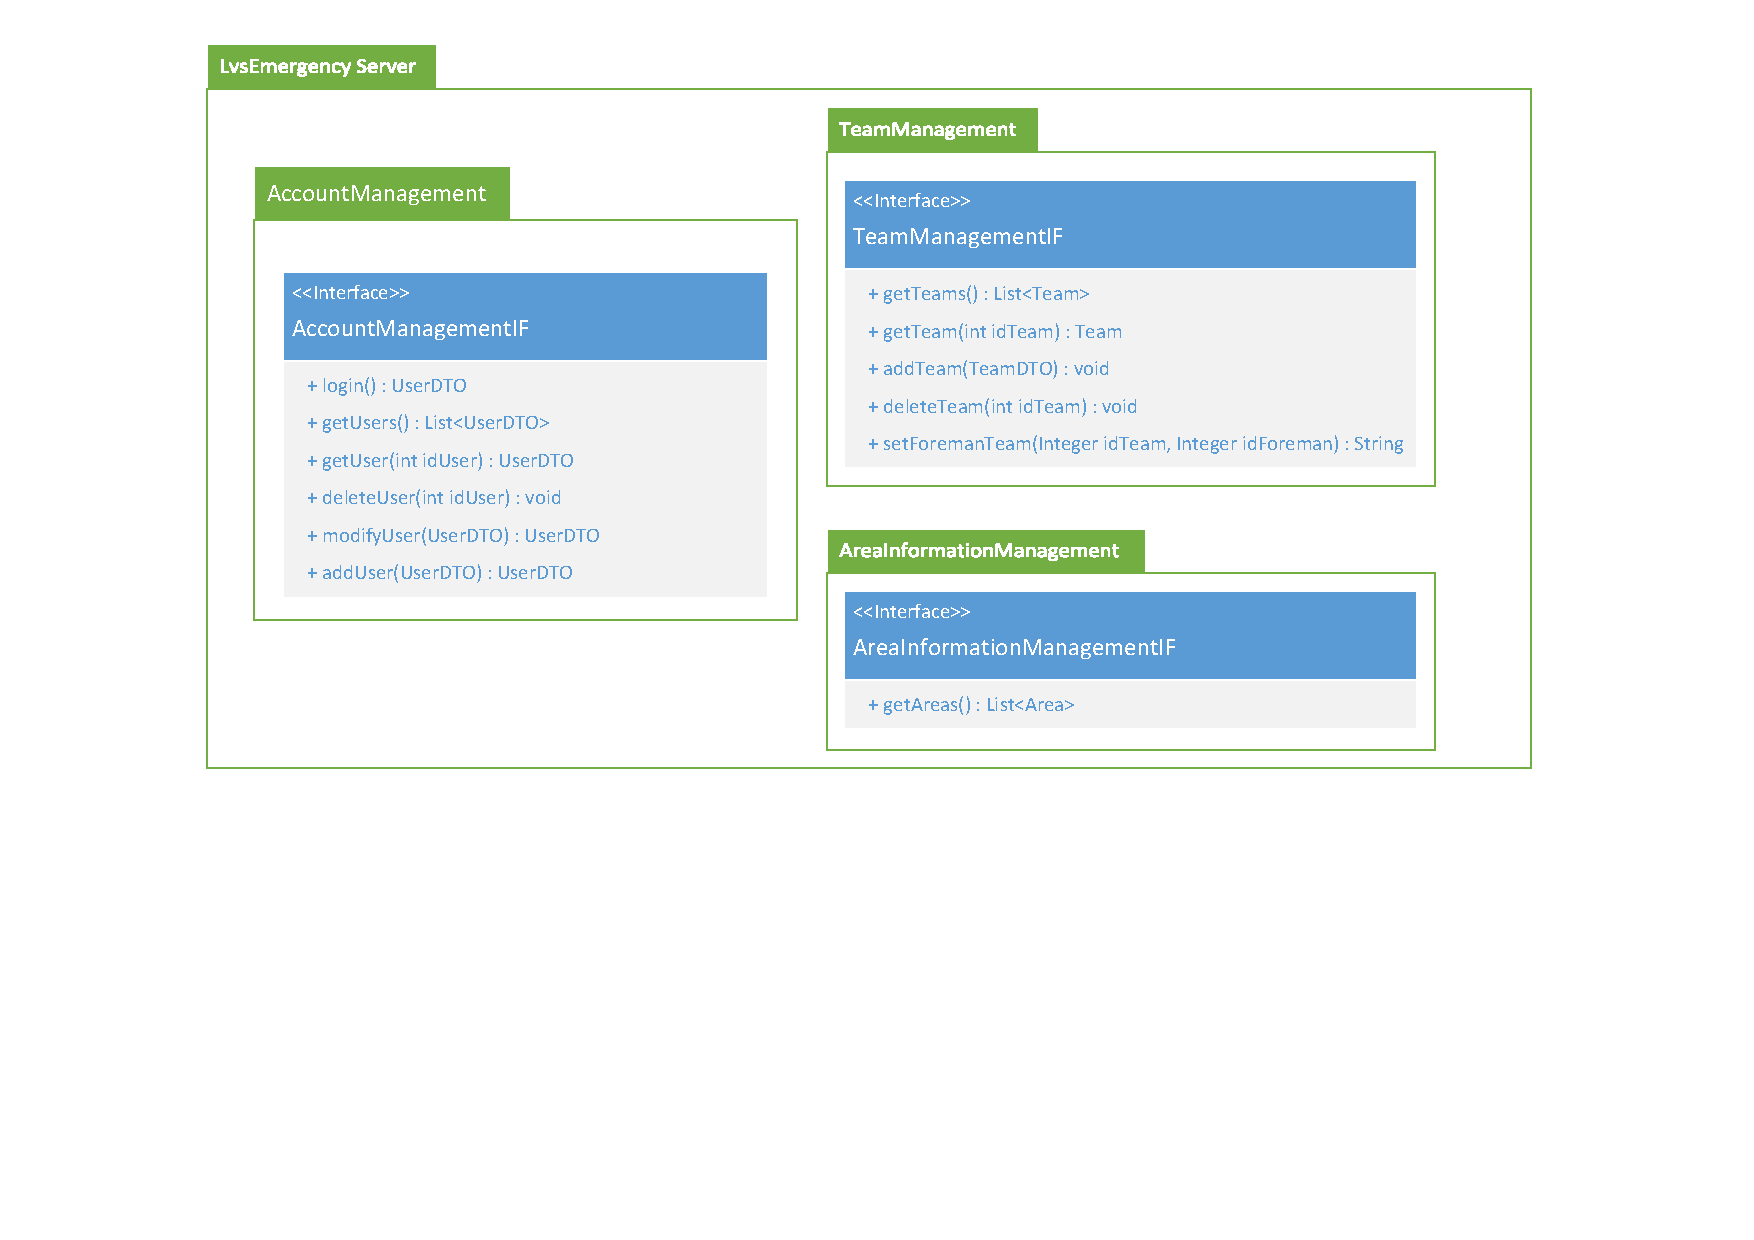
\includegraphics[width=1\linewidth]{./Iterazione 2/OtherFiles/UML - Interface Diagram}
	\caption{Interface and Package Diagram.}
	\label{fig:InterfaceDiagram_iterazione2}
\end{figure}
